\documentclass[10pt]{article}
\usepackage{pgfplots}
\usepackage{amsmath, amsfonts, amssymb, bm, color, graphicx}
\usepackage{algorithm2e, nicefrac}
\usepackage[per-mode=symbol]{siunitx}
\usepackage[paperwidth=16cm,paperheight=7cm,lmargin=0in,rmargin=0in,tmargin=0.0in,bmargin=0.in]{geometry}
\usetikzlibrary{positioning, shapes, calc, arrows}

\pgfplotsset{compat=newest}

\newlength{\figwidth}
\setlength{\figwidth}{7cm}

\begin{document}
\centering
\begin{tikzpicture}[font=\footnotesize,
    stagnate/.style={circle, draw=black, inner sep=0pt, minimum width=1em},
    frame/.style={anchor=north west, inner sep=0pt},
    sep/.style={draw=black!50!white, thick, densely dashed, shorten <= -1em, shorten >=0pt},
    time/.style={draw=none, text=black, fill=white,anchor=north west},
    dx/.style={rotate=90,anchor=south,draw=none, inner sep=3pt},
    dt/.style={anchor=south,draw=white, inner sep=3pt},
    vert_arr/.style={<->, draw=black, shorten <= 0pt, thick,shorten >= 0pt},
    scale_style/.style={text=black, fill=white, draw=black,thick, midway},
    nx_arr/.style={<->, very thick, draw=black, shorten <= 0pt, shorten >= 0pt},
    nx_style/.style={fill=white, draw=none, text=black, midway},
    lab/.style={fill=none, draw=black, text=black, anchor=north east}
  ]

  
  \node[frame,alias=1000] at (0,0)             {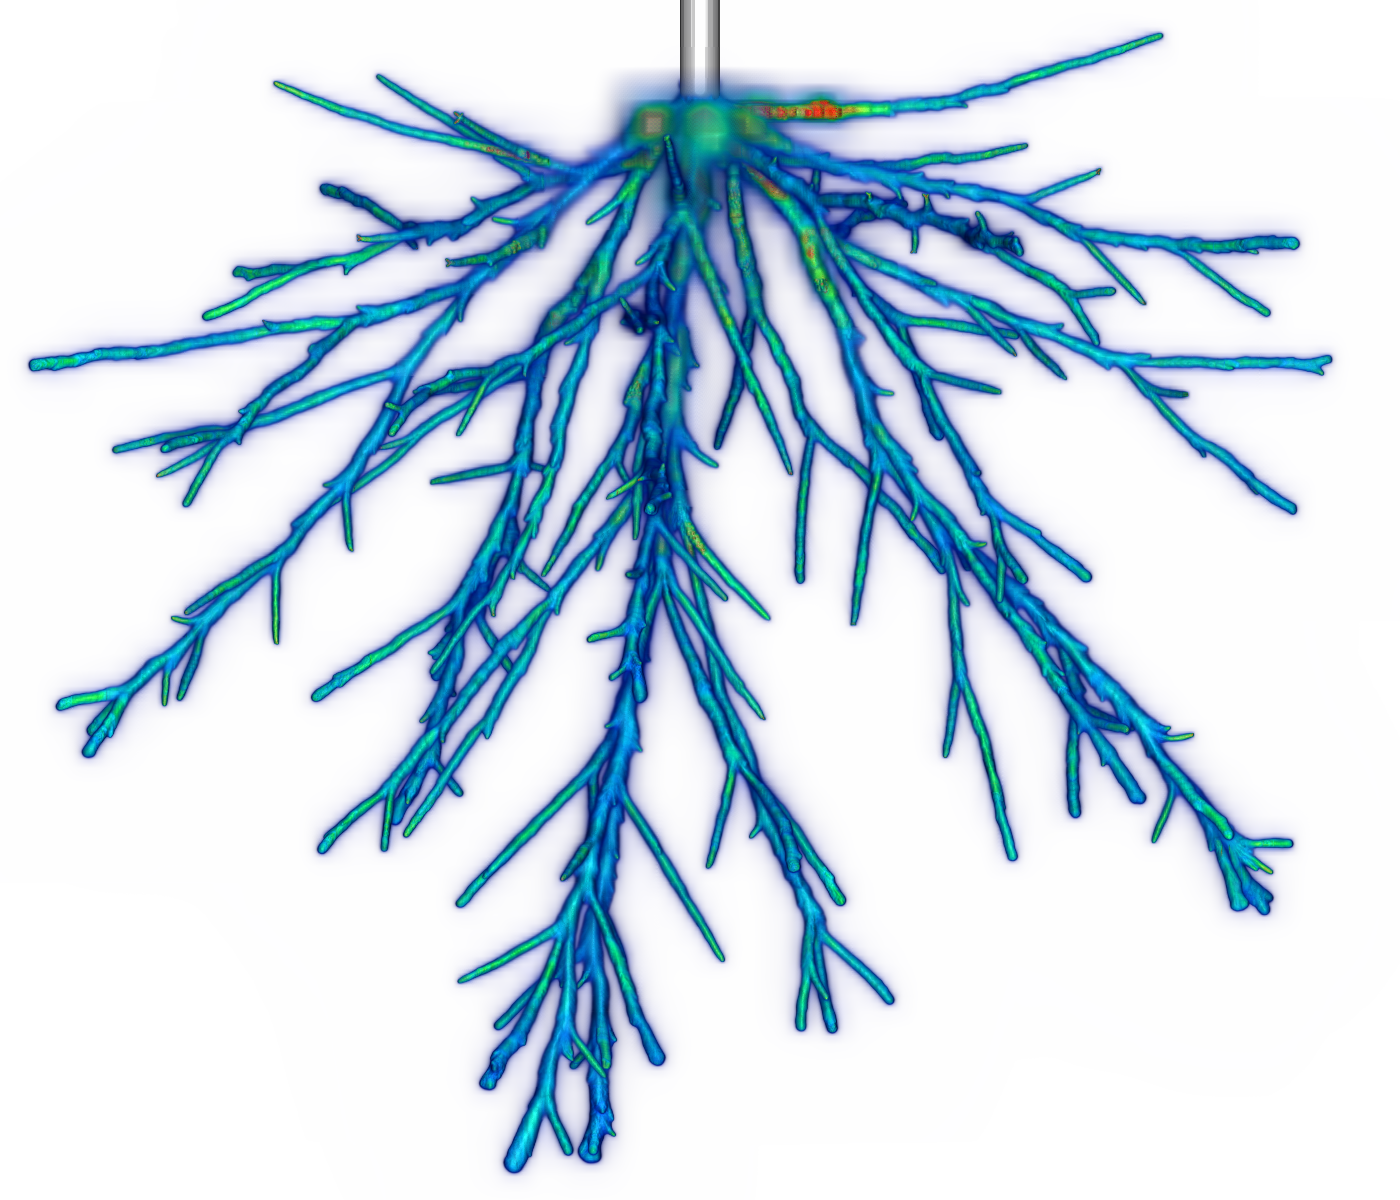
\includegraphics[width=\figwidth]{SideView}};
  \node[frame,anchor=north west,alias=2000] at (1000.north east) {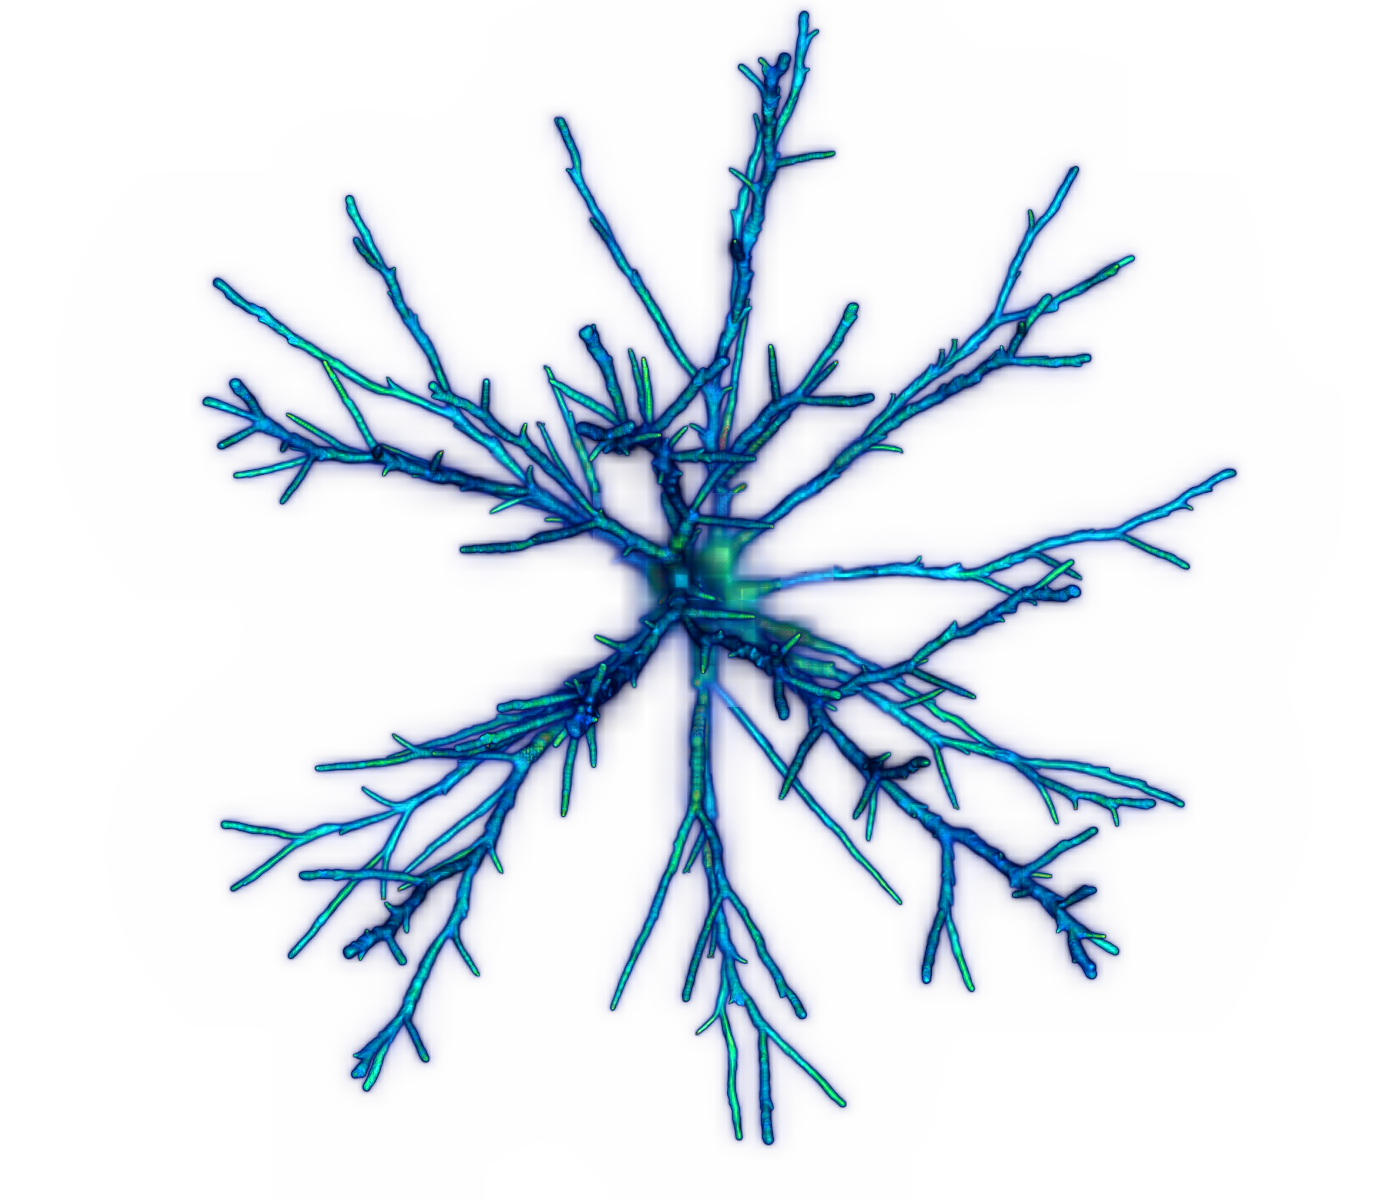
\includegraphics[width=8cm]{ViewInto}};

  \node[time] at(1000.north west) {a)};
  \node[time] at(2000.north west) {b)};
  
  \draw[sep] (2000.north west) -- (2000.south west);


  %% \draw[vert_arr] ([xshift=-2em]1000.south east) -- ++ (0,5.25) node [scale_style] {\SI{30}{\milli\meter}};  
  
\end{tikzpicture}

\end{document}
